\documentclass{beamer}

%\usepackage{pgfpages} % notes
%\setbeameroption{show notes on second screen=right} % notes
% for notes

\usepackage{Res/presento}
\setbeamercolor{background canvas}{bg=colorlgray}
\setbeamercolor{normal text}{fg=colorhgray}

\usepackage{textpos}
\setlength{\TPHorizModule}{1cm}
\setlength{\TPVertModule}{1cm}
% for textblock

\usepackage{amsmath, amsfonts, amssymb}
\usepackage{graphicx, tikz}

\graphicspath{{Res/}}

\begin{document}
    \begin{frame}[plain]
        \vfill
        \largetext{
            \color{orange}{Dimitrije Glukčević  \\
            \setnote{dimchee90@gmail.com}}
        }
        \vfill
        \largetext{\color{colorblue}
            Da li je moguće smestiti Jokića u kutiju?
        }
        \setnote{Letnji seminar za mlađe polaznike, Petnica 2021}
        \vfill
        \scalebox{0.5}{\input{Res/pmf.pdf_tex}}
        \vfill
        \begin{tikzpicture}[remember picture,overlay]
            \node[yshift=-0.5cm,anchor=north east] at (current page.north east) {
                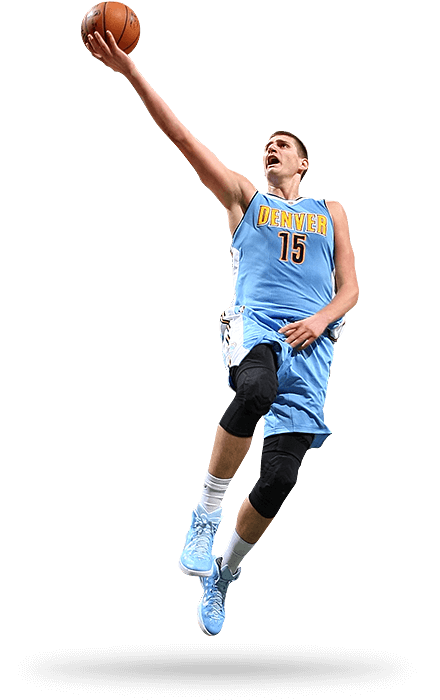
\includegraphics[height=0.8\textwidth]{Jokic/Jokic_ceo}
            };
        \end{tikzpicture}
    \end{frame}

    \begin{frame}{Priče o superherojima}
        \note{test}
        .... Neke slike (i na kraju Jokić)
    \end{frame}
    \begin{frame}{Šta to pokušavamo?}
        \begin{columns}
        \begin{column}{0.5\textwidth}
            Jokić: \begin{itemize}
                \itemR Težina - 129kg
                \itemR Visina - 2.11m
            \end{itemize}
            Standardna kutija: \begin{itemize}
                \itemR 24in x 24in x 12in
            \end{itemize}
            Dodatni uslovi: \begin{itemize}
                \itemR Kutija mora da bude zatvorena
                \itemR Vreme u kutiji je nebitno!
                \itemR Nećemo da naškodimo Jokiću!
            \end{itemize}
        \end{column}
        \begin{column}{0.5\textwidth}
            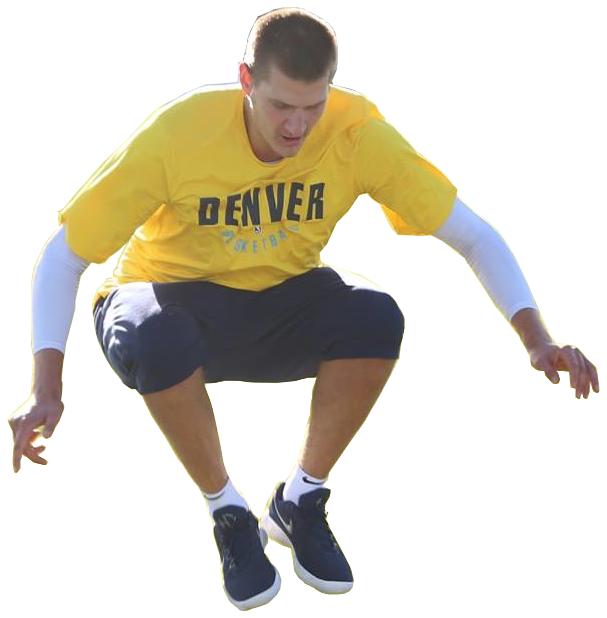
\includegraphics[height=0.4\textheight]{Jokic/Jokic_skok} \\
            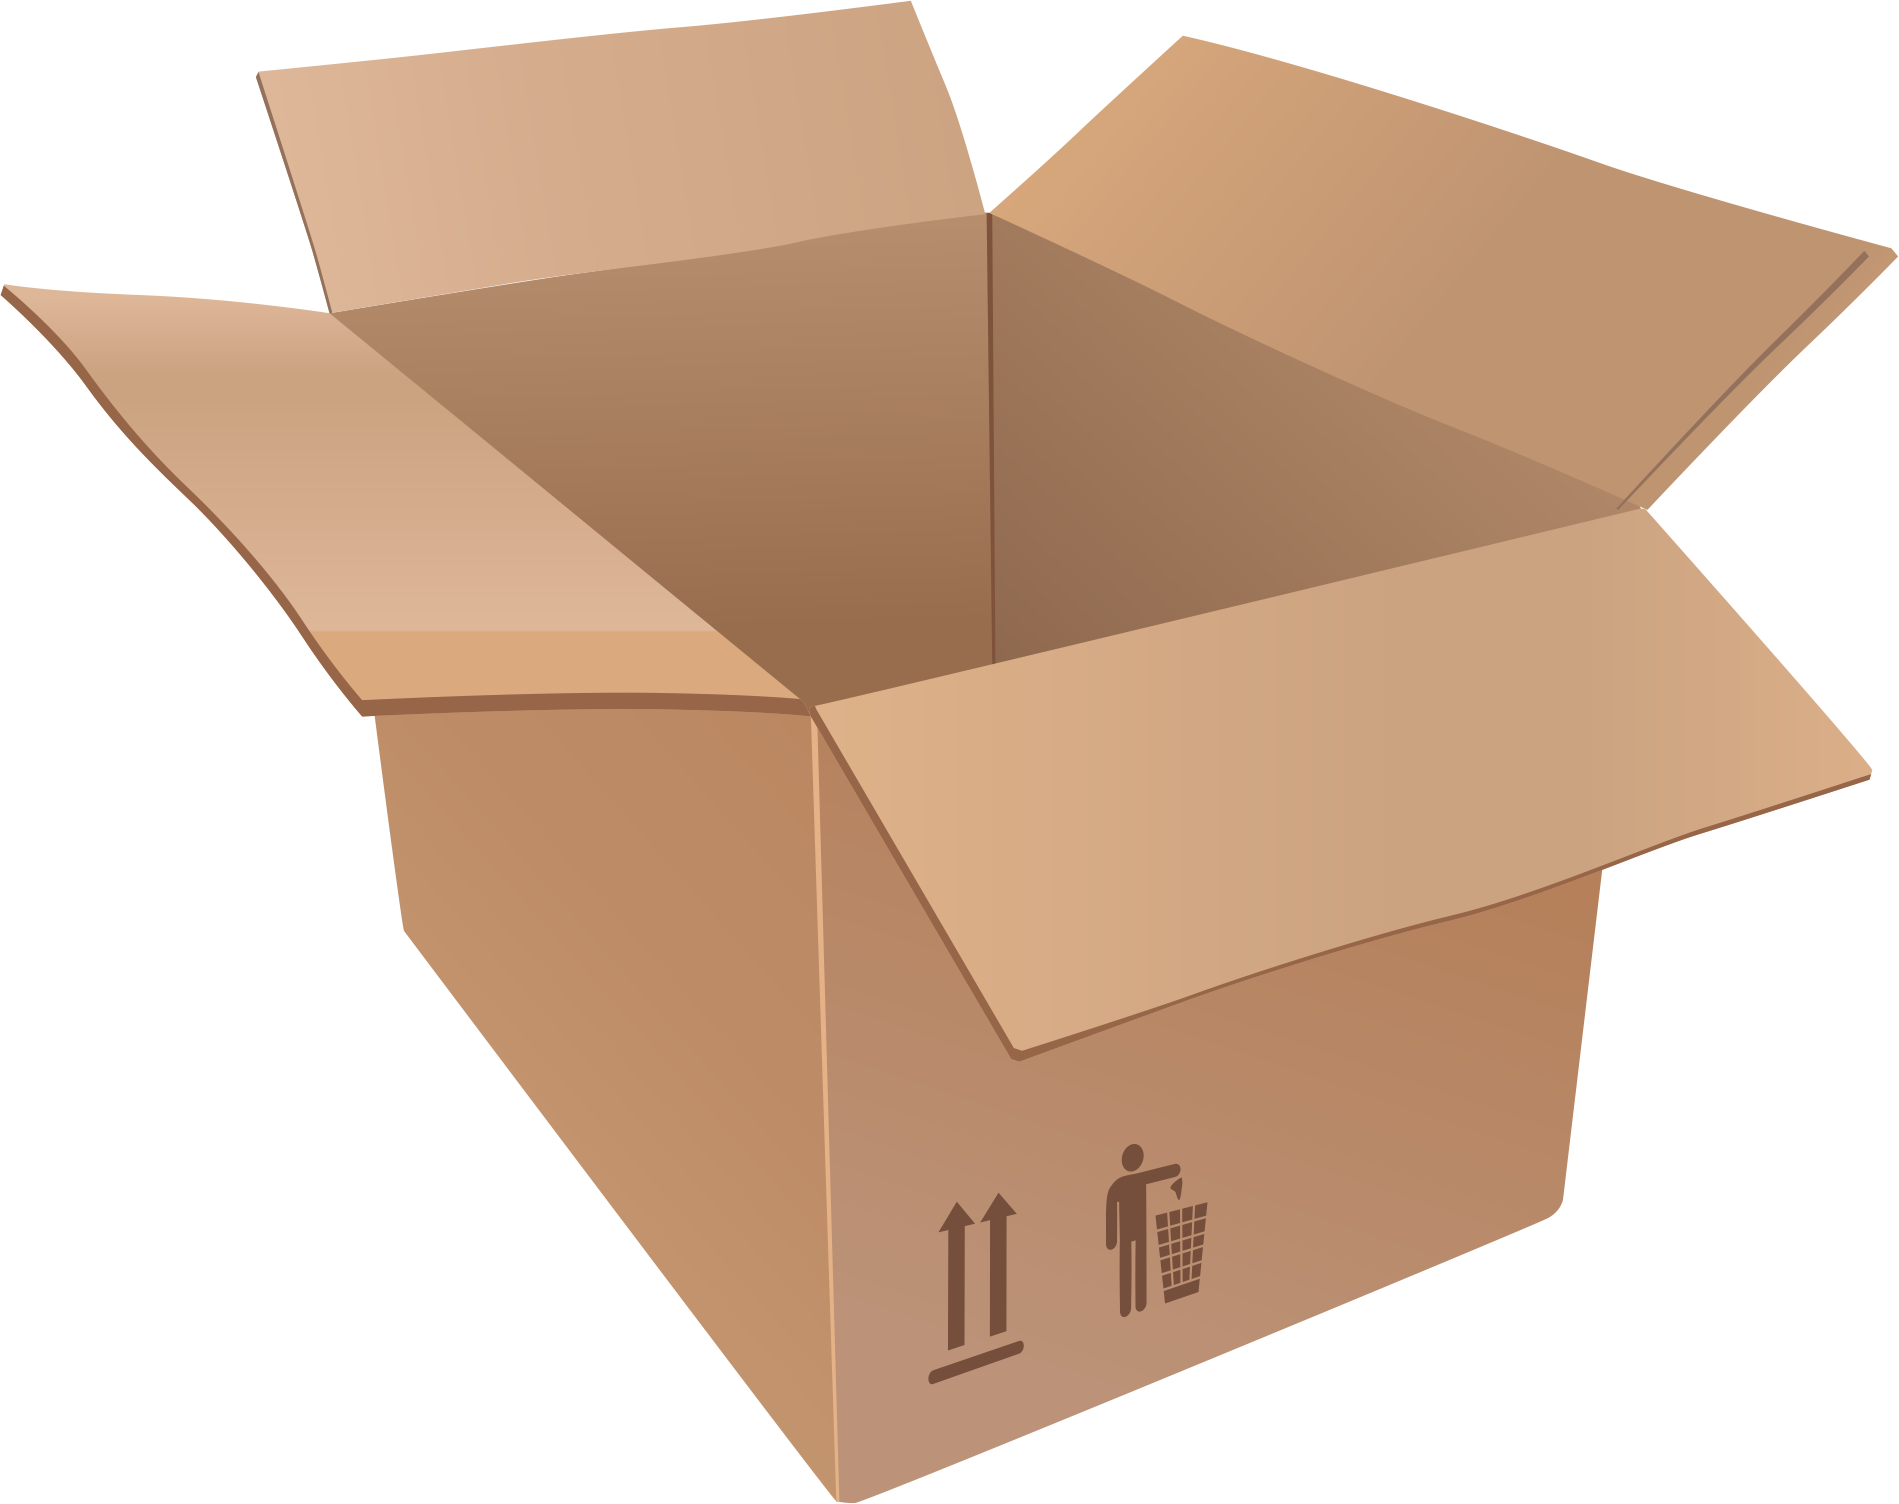
\includegraphics[height=0.3\textheight]{box}
        \end{column}
        \end{columns}
        \note{
            Šta to Jokić može a mi ne možemo?
            Dobro, zapravo ima puno toga ali
            idalje ne može da stane u kutiju
            Kao u dosta filmova poenta predavanja
            će biti da svi mi (teoretski) imamo supermoći
        }
    \end{frame}
    \framepic{reflection}{
        \frametitle{Kretanje}
        \note{
            ? Sta znaci da neko moze da stane u kutiju?
            Kretanjem mozemo da ga dovedemo u polozaj
            tako da se nalazi u kutiji
            ? Šta je to kretanje?
            ? Zasto Jokić ne moze da stane u kutiju?
            Jednoznačna transformacija koja održava rastojanje
            se naziva izometrija

            Transformacije koje očuvavaju skalarni proizvod nazivaju
            se ortogonalne (lako se predstavljaju preko matrica)

            Svaka izometrija može da se predstavi kao kompozicija
            ortogonalne transformacije i translacije. (polarni identitet)

            Ako se dve vrednosti dve izometrije poklapaju u neke četiri
            nekomplanarne tačke, onda su one jednake.
            (Dokaz: Ako se razlikuju u tački $p$ uzmeš ravan između
            ϕ(p), ψ(p) i početne četiri budu u toj ravni)
            => Izometrija je kompozicija najviše četiri refleksije.

            Izometrije formiraju grupu, čija su kretanja podgrupa
            (one izometrije koje se sastoje od parnog broja refleksija)

            Rotacija - ref. oko dve ravni koje se seku
            Translacija - ref. oko dve paralelne ravni
            Da li neko ima ideju kako da odgovorimo na pitanje da
            li može da stane u kutiju?
        }
    }
    \framecard{Međutim Jokić može da se savija :(}
    \begin{frame}{Plivanje}
        $V_{Jokic} > \frac{129kg}{1000kg/m^3} = 0.129m^3$
        $V_{Kutija} = 24in \cdot 24in \cdot 12in \cdot (0.0254 m/in)^3 < 0.114m^3$
        $V_{Jokic} > V_{Kutija}$ \\
        \note{
            Kako nam je poznata masa Jokića, a znamo da (kao čovek) pluta
            na vodi možemo da procenimo njegovu zapreminu i da je uporedimo
            sa zapreminom kutije
        }
        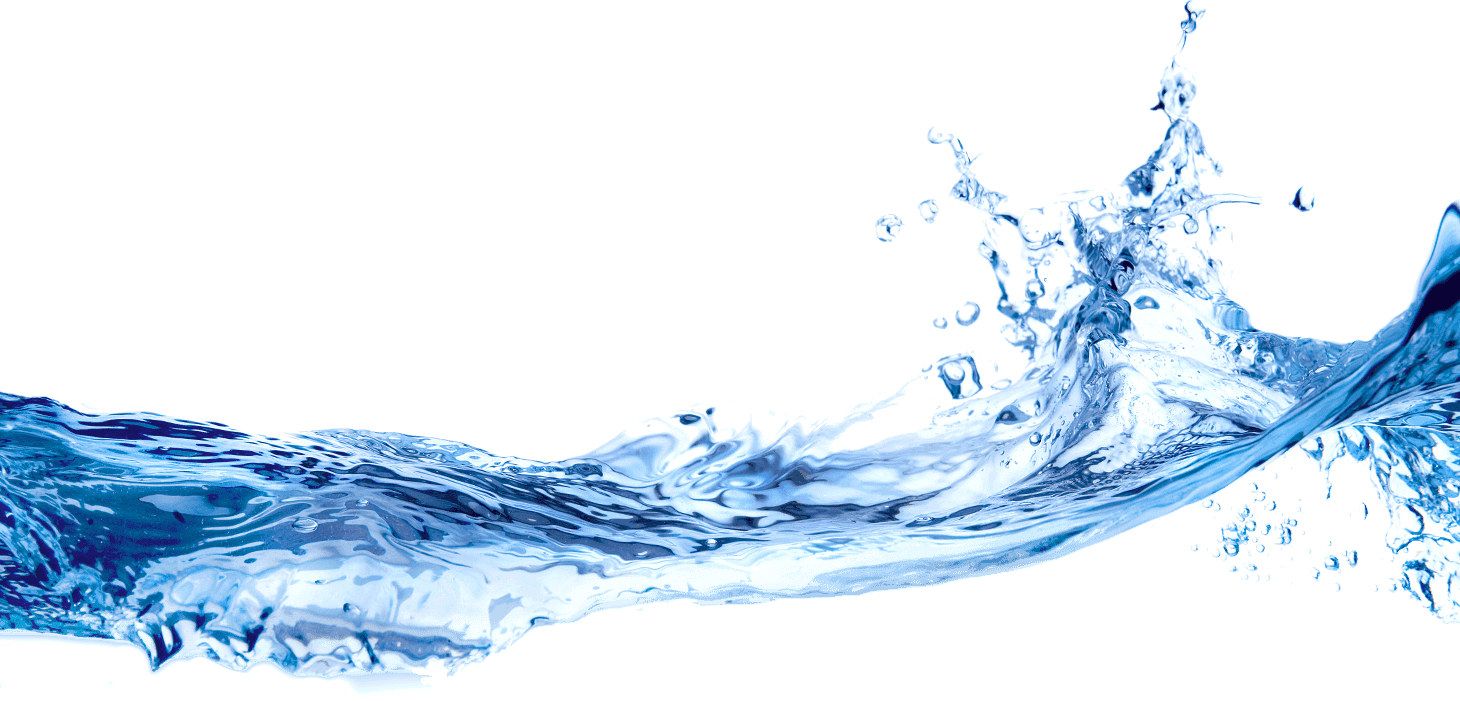
\includegraphics[width=\textwidth]{water}
    \end{frame}
    \framecard{\hugetext{Šta sad?}}
    \framepic{Jokic/Jokic_stajebreovo}{
        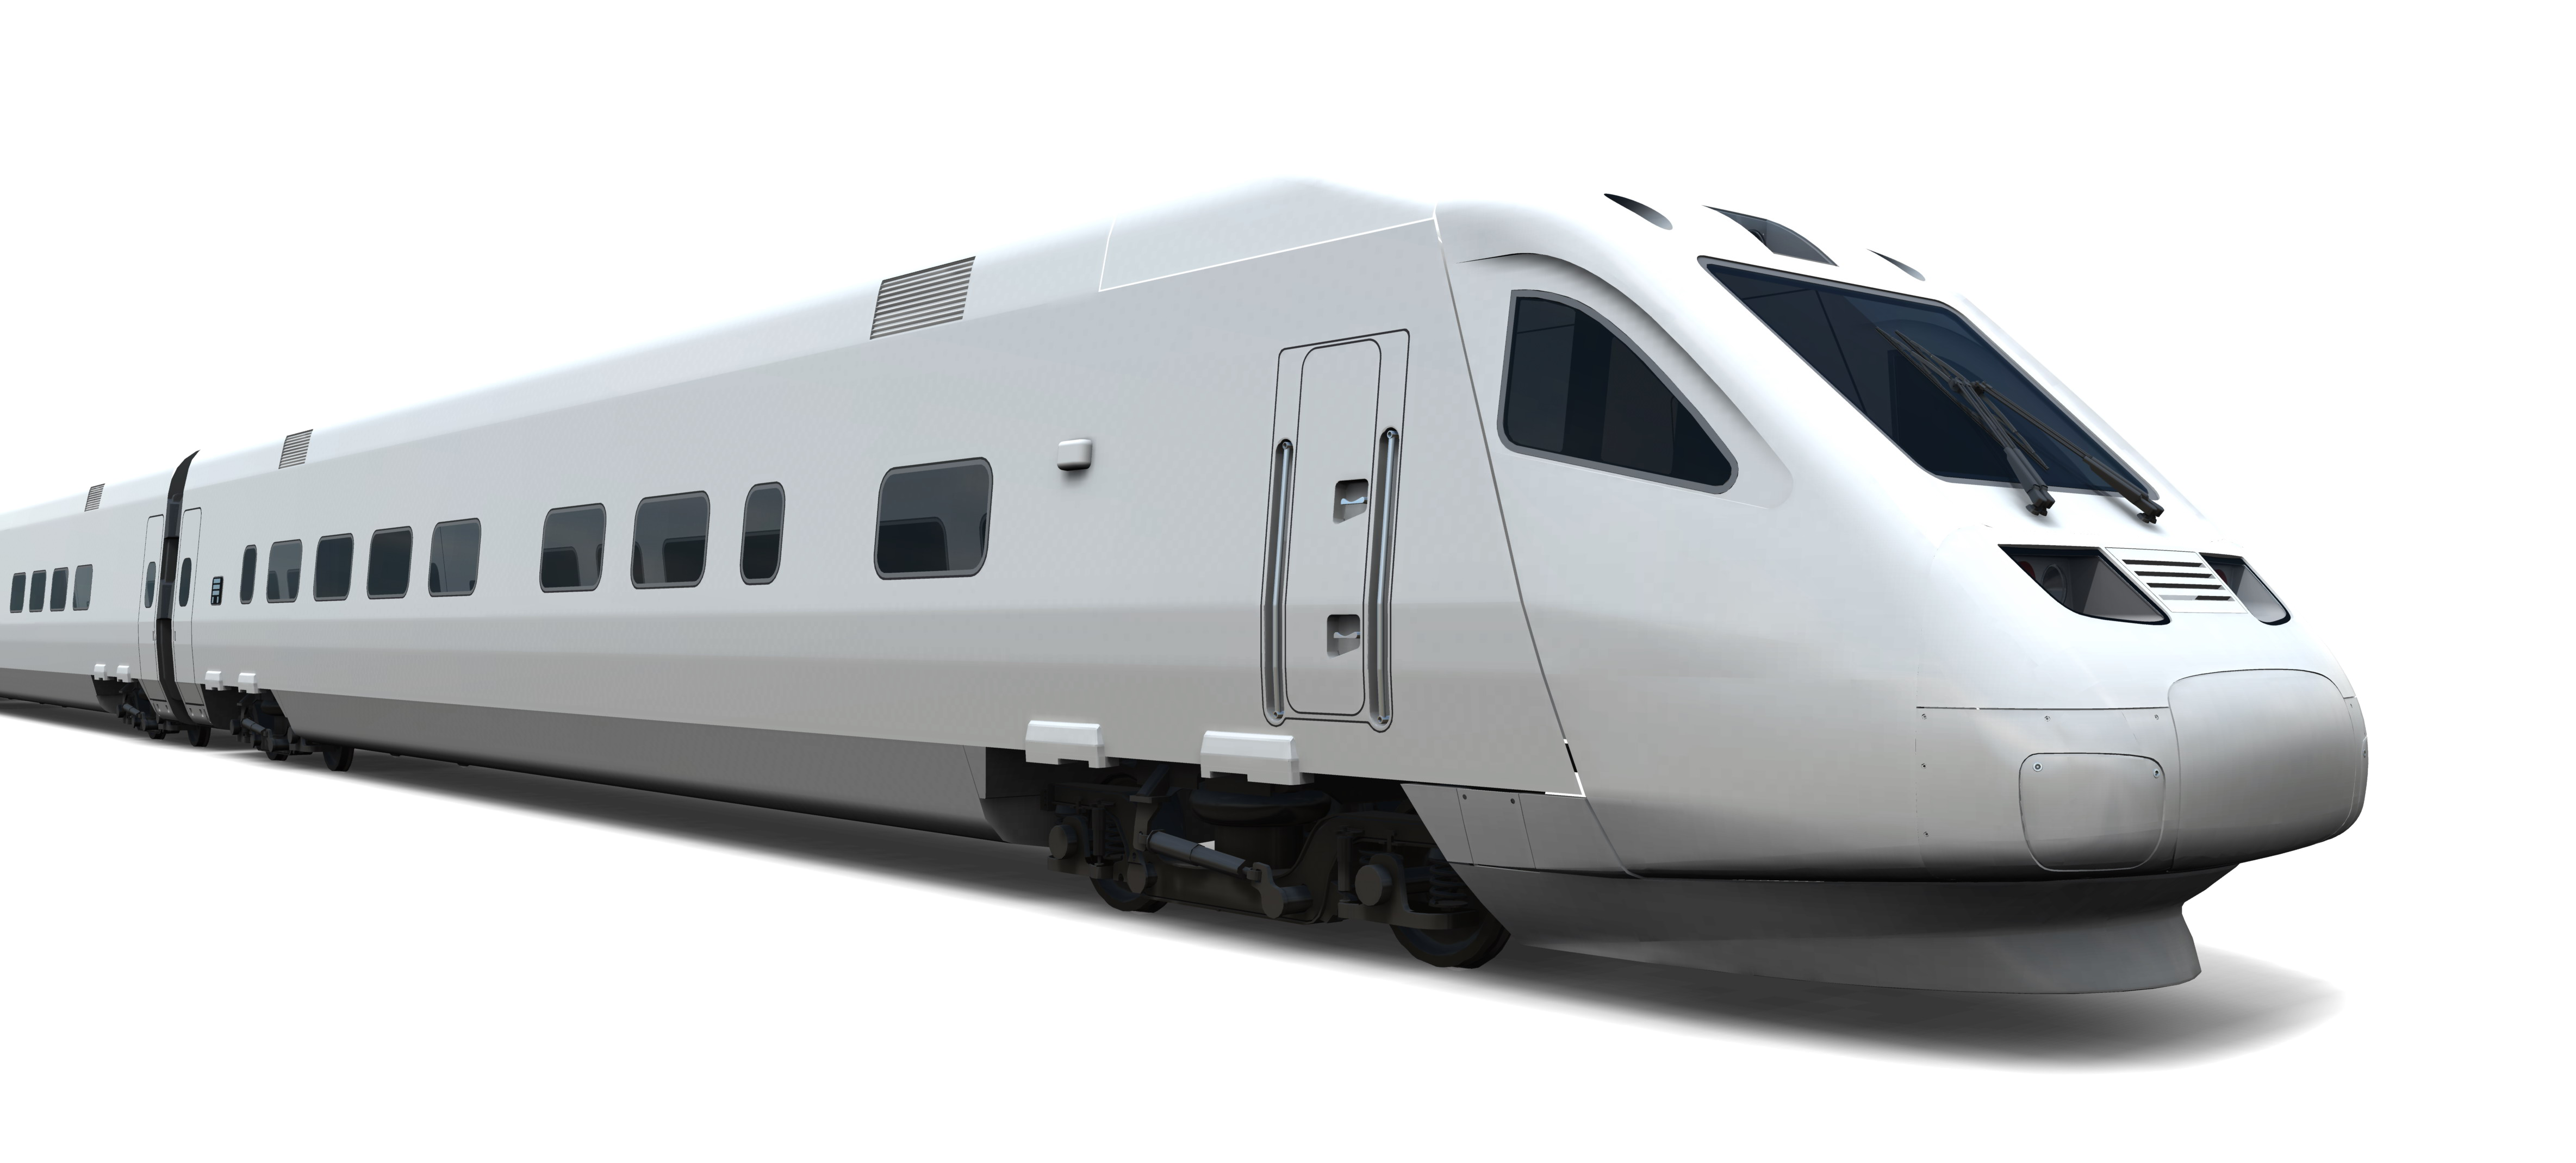
\includegraphics[height=0.15\textheight]{train}
        \begin{textblock}{2}(9,-2)
            $ t' = t \frac 1 {\sqrt{1 - \frac {v^2} {c^2}}} $
        \end{textblock}
        \begin{textblock}{2}(9,2)
            $$ E = mc^2 $$
        \end{textblock}
        \begin{textblock}{3}(1,3)
            $ l' = l {\sqrt{1 - \frac {v^2} {c^2}}} $
        \end{textblock}
        \note{
            ... Slika na kojoj se vidi zašto je put različit
            Prvo priča o vozovima, intuitivno šta je to Ajnštajn smislio
            Brzina svetlosti konstantna
            Različita vremena
            Kontrakcija dužine, dilatacija vremena...
        }
    }
    \begin{frame}{Cliff Hanger}
        Ako se Jokić kreće brzinom $v$ koja je blizu brzine svetlosti
        desiće se kontrakcija njegove visine i na kratko ćemo moći da
        ga smestimo u kutiju.
        \note{
            Da li vam ovo deluje zanimljivo?
            Koliko vam ovo deluje kao naučna fantastika?
        }
        \begin{tikzpicture}[remember picture,overlay]
            \node[anchor=south east, yshift=-5pt, xshift=-20pt] at (current page.south east) {
                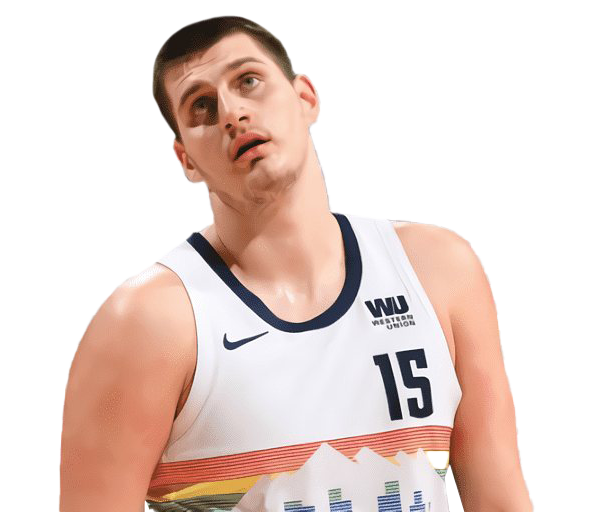
\includegraphics[height=3.0cm]{Jokic/Jokic_realy}
            };
        \end{tikzpicture}
    \end{frame}
    \framecard{\hugetext{Problem?}}
    \note{
        Za Jokića je pak kutija doživela kontrakciju dužine,
        dakle u kutiju ne može da mu stane ni glava
    }
    \framepic[0.3]{ruler}{
        Da li možemo da izdvojimo nešto fundamentalnije što bi nam
        pomoglo (kao matematičarima) da lakše razmatramo ovaj problem?
    }
    \note{
        Crtanje grafika (s od t) po tabli (podcećanje na fiziku iz osnovne)
        Izvođenje Lorencovih transformaciija
        Crtanje po tabli, objašnjavanje invarijantnosti dužine u
        Euklidskoj geometriji, izvođenje invarijantnosti
        prostor-vremenskog intervala

        Zasnivanje geometrije Minkovskog na invarijantnosti
        dužine prostor vremenskog intervala (i zašto ona nije baš
        dužina, pravo vreme posmatrača...)

        Crtež na kome se vidi da va dužina nije baš intuitivna
        (tačke na istom 'rastojanju' od koordinatnog početka obrazuju
        hiperbolu)
        Ispada da su Lorencove transformacije zapravo samo
        hiperboličke rotacije

        Izometrije slikaju pravu u pravu.
        (uzmu se prave p(e_1, e_2) i p'(ϕ(e_1), ϕ(e_2)))

        Teorema o 3 događaja za ravan Lorenca i Minkovskog
        (dokaz isti ko za euklidsku ravan)

        Teorema o 4 refleksije za ravan Lorenca i Minkovskog
        (refleksije nisu bas jednostavne kao u Euklidskoj)
    }
    \framepic{resenje}{
        \frametitle{Rešenje}
        \note{
            Kada se posmatraju događaji:
            A - kada Jokić prolazi kroz kutiju tada se druga vrata otvore
            B - kada Jokić izađe iz kutije tada se prva vrata zatvore
            Kod Jokića u referentnom sistemu se oni dešavaju redosledom
            prvo A pa onda B, dok se u referentnom sistemu kutije dešavaju
            prvo B pa onda A (dakle Jokić je proveo neko vreme zatvoren :))
        }
    }
    \framepic{dominoes}{
        \frametitle{Kauzalnost}
        \note{
            Kauzalnost je relacija delimičnog poretka.
            Kauzalnost je invarijanta u odnosu na grupu Lorencovih transformacija.
            Kauzalnost je invarijantna u odnosu na grupu svih
            'fizički mogućih transformacija' i zato ih zovemo kauzalne
            izometrijske transformacije
            Kako je $c$ baš veliko, ispada da su kauzlno neuslovljeni događaji
            prostorno puno udaljeni.
        }
    }
    \begin{frame}{Potpun poredak?}
    \end{frame}
\end{document}
